\lab{Algorithms}{Eigenvalue Solvers And Markov}{Eigenvalue Solvers And Markov}
\objective{Implement the $QR$ algorithm for finding eigenvalues and learn Markov chains.}
\label{lab:EigSolve}

\section*{Eigenvalues are hard to find}

Finding the eigenvalues of $n \times n$ matrix $A$ means solving the following equation, where $x$ is a nonzero vector and $\lambda$ is a scalar.
\begin{align}
A x &= \lambda x \notag \\
A x - \lambda x &= 0 \notag \\
(A - \lambda I)x  &= 0 \label{eq:singularity}
\end{align}
Since $x$ is nonzero, \eqref{eq:singularity} means $A-\lambda I$ must be singular.
Thus $\det(A - \lambda I) = 0$.  This determinant is often notated $\det(A - \lambda I) = p(\lambda)$ and is called the \emph{characteristic polynomial} of $A$.
The roots of the characteristic polynomial are the eigenvalues of $A$.

If $A$ is $n \times n$, the degree of $p(\lambda)$ is  $n$.
Finding the roots is easy for small $n$, but it becomes difficult or impossible as $n$ increases.
Abel's Theorem  outlines the problem.

\begin{theorem}
{\bf Abel's Impossibility Theorem:} There is no general algebraic solution for solving a polynomial equation of degree $n>4$.
\label{Theorem:Abel}
\end{theorem}

Therefore, there is no method that will exactly find the eigenvalues of an arbitrary matrix.
This is a significant result. In practice it means that we often rely on iterative methods, which converge to the eigenvalues.

\section*{The Power Method}
There are many such iterative methods for finding eigenvalues. The Power Method is a simple fast way to find the largest eigenvalue and eigenvector. You begin with a vector $x_0$, that has norm 1, and do the iteration.
\[
x_{k+1}=\frac{Ax_k}{\norm{Ax_k}}
\]
it works when
\begin{itemize}
\item The matrix $A$ has a eigenvalue that is strictly greater in magnitude than its other eigenvectors.
\item your starting vector $x_0$ has a nonzero component in the direction of the eigenvector of the dominant eigenvalue.

\end{itemize}

This often converges slowly (geometric with the ration given by $\norm{\lambda_2/\lambda_1}$ but is especially useful when your matrix has all positive values because you are guaranteed to have a dominant eigenvalue and the modulus of dominant eigenvalue is often much greater than the rest of the eigenvalues so the convergence is much faster.
Whenever you have an eigenvector you can compute its corresponding eigenvalue using the Rayleigh quotient
\[
\lambda = \frac{Ax\cdot x}{x\cdot x}
\]
\begin{problem}
Write a method that takes a in matrix and a tolerance and computes its largest eigenvalue and the eigenvector. Have your starting vector be random. Use the two-norm and have the iteration stop when the maximun change of the vector is less than the tolerance. Test your function on positive matrices.
\end{problem}

\begin{comment}
An overview of the proof of the method is that you can write a matrix in Jordan Conical form $A=VJV^{-1}$ where $V$ is the matrix of the generalized eigenspaces. But the first column is is the eigenvector corresponding to largest eigenvalue and $J$ is a upper trianglar matrix of eigenvalues and ones.  Note that $A^k=VJ^kV^{-1}$. The limit as $k \rightarrow \infty$ of $(\frac{1}{\lambda_1}J)^k$ is a matrix of all zeros except for a one in the upper right hand corner. So $(\frac{A}{\norm{A}})^k \approx VJ^kV^{-1}$ So the largest eigenvalue dominates.
\end{comment}

The down side is that it only finds the largest eigenvector and eigenvalue. The next algorithm finds more eigenvalues.

\section*{The $QR$ algorithm}


We will explore one of the simplest: the $QR$ algorithm.
The following recurrence describes the $QR$ Algorithm in its most basic form:
\begin{equation*}
A_0 = A, \quad A_k = Q_k R_k, \quad A_{k+1} = R_k Q_k
\end{equation*}
where $Q_k, R_k$ is the $QR$ decomposition of $A_k$.
Yes, it's as easy as it looks.
All this algorithm does at each step is find the $QR$ decomposition of $A_k$ and multiply $Q_k$ and $R_k$ together again but in the opposite order.
How does this simple algorithm find the eigenvalues of $A$?

\begin{comment}
\begin{problem}
\label{problem:similarity proof}
Prove that $A_{k+1} \sim A_k$ (where $\sim$ denotes matrix similarity).
Then prove that $A_n \sim A$ for all $n$.
\end{problem}
\end{comment}

Observe that $A_{k+1} \sim A_k$ (where $\sim$ denotes matrix similarity).
Then $A_n \sim A$ for all $n$.
This statement shows that $A_n$ has the same eigenvalues as $A$.
Preservation of eigenvalues is the first important feature that makes the algorithm work.
The other important feature is that each iteration of the algorithm effectively transfers some of the``mass" from the lower to the upper triangle.
Under very general conditions, $A_n$ will converge to a matrix of the form

\begin{equation*}
\label{eq:Schur form}
S =
     \begin{pmatrix}
          S_1 &* & \cdots & * \\
           0     &S_2  &  \ddots & \vdots \\
           \vdots  & \ddots & \ddots & *  \\
           0 & \cdots & 0 & S_m
    \end{pmatrix}
\end{equation*}
where $S_i$ is either a $1 \times 1$ or a $2 \times 2$ matrix.
For most matrices $A$, all the $S_i$ will be $1 \times 1$, so $S$ will be an upper triangular matrix.
In this case, $S$ is called the \emph{Schur form} of $A$.
The eigenvalues of $A$ are on the main diagonal of $S$.

The only case where $S$ is not upper triangular is when $A$ is a real but not symmetric matrix.
In this case, though $A$ is real, it may have complex eigenvalues.
These eigenvalues occur in complex conjugate pairs.
Each of these pairs corresponds to a $2 \times 2$ block in $S$, where the eigenvalues of the $2 \times 2$ block are the complex conjugate pair of eigenvalues of $A$.
In this case, $S$ is called the \emph{real Schur form} of $A$.

\subsection*{Hessenberg preconditioning}

Recall that an upper Hessenberg matrix looks like
\[
\begin{pmatrix}
* & * & * & \cdots & * \\
* & * & * & \cdots & * \\
0 & * & * & \cdots&* \\
\vdots & & \ddots & \ddots & \vdots \\
0 & \cdots & 0 & * & *\\
\end{pmatrix}
\]
and that every matrix is similar to an upper Hessenberg matrix.
Hessenberg reduction also preserves eigenvalues.
It is a good idea to reduce to Hessenberg form before continuing with the $QR$ algorithm.
You'll converge to the Schur form faster this way, since Hessenberg matrices are already close to upper triangular.

\begin{problem}
Write a function \li{qrSolver} that implements the QR algorithm as described above. Use the QR decomposition built into \li{scipy.linalg}.
Have your function accept a real-valued $n \times n$ matrix $A$, a number of iterations, and a tolerance number,
and return the corresponding estimate for all the eigenvalues of $A$.
Note that you will need to find the eigenvalues of the $2 \times 2$ $S_i$ directly, whenever there are any.
\end{problem}

Reducing the matrix to Schur form also has the added benefit that each iteration for an $n \times n$ array can be computed in $\mathcal{O} \left( n^2 \right)$ time instead of $\mathcal{O} \left( n^3 \right)$.
One algorithm for computing the QR decomposition of an upper Hessenberg matrix was discussed in Lab \ref{lab:givens}.
This works since $Q$ in the QR factorization of an upper Hessenberg matrix is also upper Hessenberg, the product $R Q$ also turns out to be upper Hessenberg.

\begin{comment}
\begin{problem}
\label{prob:QR_eig_hessenberg}
Write a version of the QR algorithm that performs the QR algorithm by computing the Hessenberg form of a matrix, then computing various QR decompositions of the Hessenberg form of the matrix.
Use your solutions to \ref{prob:hessenberg} (where you computed the Hessenberg form of a matrix) and Problem \ref{prob:givens_hessenberg_modified} to do the necessary computations (where you computed the QR decomposition of a Hessenberg matrix and wrote code for multiplication by $Q$ that works in $\mathcal{O} \left( n^2 \right)$ time).
The solution to Problem \ref{prob:givens_hessenberg_modified} is especially important because it allows the compution of each QR decomposition and each $R Q = \left( Q^T R^T \right)$ in $\mathcal{O} \left( n^2 \right)$ time.
\end{problem}
\end{comment}

\begin{comment}

\begin{problem}
If $A$ is normal, its Schur form is diagonal.
For normal $A$, have your function additionally output the eigenvector corresponding to each eigenvalue.
Hint 1: Test your function on Hermitian and real symmetric matrices; they are both normal.
Hint 2: Your work in Problem \ref{problem:similarity proof} will help.
You have already made all the necessary calculations, you just need to store the information correctly.
\end{problem}

\end{comment}

\begin{problem}
Test your implementation with random matrices.
Try real-valued and symmetric matrices.
Compare your output to the output from the eigenvalue solver.
How many iterations are necessary?
How large can $A$ be?
\end{problem}

Be aware that the algorithm we coded today is a very un-optimized approach.
In practice, the QR algorithm as we have described it here is not generally used.
There is an improved version called the Implicit QR algorithm that iterates much more efficiently.

Further, the QR algorithm is not the only iterative method used to find eigenvalues.
Arnoldi iteration is similar to the QR algorithm but exploits sparsity.
Other methods include the Jacobi method and the Rayleigh quotient method.

As a final note, it is important to remember that eigenvalue solvers can be wrong, particularly for matrices that are ill-conditioned. Convergence is not unconditionally guaranteed. 

\section*{Markov Chains}
A Markov Chain describes a particular type of random process that
undergoes a sequence of transitions among various states. It is
characterized by the fact that all relevant information is related to its current state.
We can easily model this process using matrices.
We will start with a simple example of a frog jumping from one lily pad to another.

Suppose Fredo the frog jumps around between the three lily pads 1, 2, and 3.
These three pads are taken as the possible \emph{states} of the system, and the
lily pad on which Fredo is presently sitting is the \emph{current state}.
If Fredo is on lily pad 1 and jumps, there is a 25\% chance that it will land back on lily pad 1, a 25\% chance that it will land on lily pad 2, and a 50\% chance that it will land on lily pad 3.
We can find similar probabilities if he starts on lily pad 2 or 3.
Such probabilities are known as the \emph{transition probabilities}.
In figure \ref{fig:markov1} we have a transition diagram that reflects the various probabilities of jumping from one lily pad to another.

\begin{figure}[h]
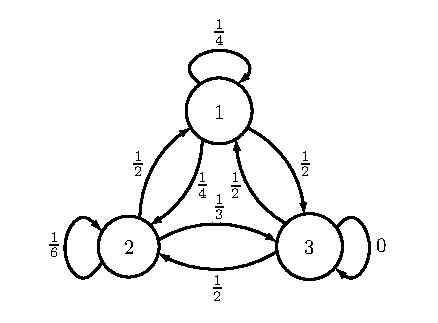
\includegraphics[width=\textwidth]{markov1}
\caption{Transition diagram for Fredo the Frog}
\label{fig:markov1}
\end{figure}

We can convert our transition diagram into a transition matrix, where the $(i,j)$-entry of the matrix corresponds to the probability that Fredo jumps from the $j^{th}$ lily pad to the $i^{th}$ lily pad (where $1$ is the first lily pad, $2$ is the second, and so on).
The transition matrix is
\[
A = \begin{pmatrix}
1/4 & 1/2 & 1/2\\
1/4 & 1/6 & 1/2\\
1/2 & 1/3 & 0
\end{pmatrix}
\]
Note that all of the columns add up to one.
This is important.

If Fredo is on lily pad 1, where will it be after two jumps?
By multiplying the matrix $A$ by itself, we have (approximately)

\[
A^2 = \begin{pmatrix}
0.4375 & 0.3750 & 0.3750\\
0.3542 & 0.3194 & 0.2083\\
0.2083 & 0.3056 & 0.4167
\end{pmatrix}
\]
From this, we infer that there is a 43.75\% chance the frog will still be on lily pad 1 after two jumps.
Note that it might have jumped from 1 to 1 to 1, denoted $1 \rightarrow 1 \rightarrow 1$, or it could have jumped to one of the other lily pads and then back again, that is, either $1 \rightarrow 2 \rightarrow 1$ or $1 \rightarrow 3 \rightarrow 1$.
In addition, there is a 35.42\% chance it will be on lily pad 2 and a 20.83\% chance that it will be on lily pad 3.
Using Python, we can type in our transition matrix and see where Fredo will be after 5, 10, 20 or 100 jumps.

\begin{lstlisting}
#Remember, the 1.'s in the numerator force floating point division
>>> A = np.array([[1./4,1./2,1./2],[1./4,1./6,1./2],[1./2,1./3,0]])
>>> np.linalg.matrix_power(A,5)
>>> np.linalg.matrix_power(A,10)
>>> np.linalg.matrix_power(A,20)
>>> np.linalg.matrix_power(A,100)
\end{lstlisting}

Note that as we take higher powers it appears that the limit goes to
\[
A^\infty = \begin{pmatrix}
0.4 & 0.4 & 0.4\\
0.3 & 0.3 & 0.3\\
0.3 & 0.3 & 0.3
\end{pmatrix},
\]
and this can, in fact, be proven carefully.
This means that after several jumps, the probability that we will find Fredo on a given lily pad will have nothing to do with where he started initially.


We can generalize this notion beyond that of frogs and lily pads.
Let the state distribution of our system be represented by a probability vector
\[
\x = \begin{bmatrix}
x_1\\
x_2\\
\vdots\\
x_n
\end{bmatrix}
\]
where each entry represents the probability of being in that state.
Note that each entry is non-negative and the sum of all the entries adds up to one.
For example, in the frog example, if we know initially that it is on lily pad 1, then we have the probability vector
\[
\x_0 = \begin{bmatrix}
1\\
0\\
0
\end{bmatrix}
\]
because we know for certainty (100\%) that Fredo is in the first state.
After one jump, we have
\[
\x_1 = A \x_0 = \begin{bmatrix}
0.25\\
0.25\\
0.50
\end{bmatrix}
\]
After two jumps, we have
\[
\x_2 = A \x_1 = A^2 \x_0 = \begin{bmatrix}
0.4375\\
0.3542\\
0.2083
\end{bmatrix}
\]
After a large number of jumps $(n>>1)$, we have
\[
\x_n = A \x_{n-1} = \dots = A^n \x_0 \approx \begin{bmatrix}
0.4\\
0.3\\
0.3
\end{bmatrix}
\]
Since all of the columns are the same for $A^\infty$, it follows that for any initial probability vector $\x_0$, we get the same limiting output, or in other words, all initial vectors converge to the same point, call it $\x_\infty$.
Moreover, we have that
\[
\x_\infty = A \x_\infty
\]
This is called a \emph{stable fixed point}.
How can we check that a stable fixed point exists?

Notice this is just the power method iteration without dividing by the norm. Since the all of the columns of $A$ sum to one and $x_0$ sums to one the one norm of $Ax_k=1$ for all $k$. So this goes to a stable fixed point and that fixed point turns out to be the eigenvector corresponding to the largest eigenvalue. Note that all the columns sum up to one and that a matrix and its transpose have the same eigenvalues. It can be shown that if all the rows of a positive matrix sum to the same number that number is the largest eigenvalue and the corresponding eigenvector is the one vector. So the $A.T$ has the eigenvalue $\lambda=1$ so $A$. So for any Markov chain the largest eigenvalue will be $\lambda=1$.

\section*{Example}
Consider the Markov chain given by
\[
A = \begin{pmatrix}
0.5 & 0.3 & 0.4\\
0.2 & 0.2 & 0.3\\
0.3 & 0.5 & 0.3
\end{pmatrix}.
\]

We do this via Python:
\begin{lstlisting}
>>> from scipy import linalg as la
>>> A = np.array([[.5,.3,.4],[.2,.2,.3],[.3,.5,.3]])
>>> V = la.eig(A)[1]
\end{lstlisting}
Note that the entries in the $\lambda=1$ eigenvector do not generally add up to one.
Indeed, any multiple of an eigenvector is an eigenvector.
So we need to multiply it by the appropriate constant so that all of the entries add up to one.
\begin{lstlisting}
>>> x = V[:,0]
>>> x = x/np.sum(x);x
array([ 0.41836735,  0.23469388,  0.34693878])
\end{lstlisting}
We can check this answer by taking $A$ to a high exponent, say $A^{100}$.

\begin{problem}
Suppose a basketball player's success at shooting free throws can be described with the following Markov chain
\[
A = \begin{pmatrix}.75&.50\\.25&.50\end{pmatrix}
\]
where the first state corresponds to success and the second state to failure.
\begin{enumerate}
\item If the player makes his first free throw, what is the probability that he also makes his third one?
\item What is the player's average free throw percentage?
\end{enumerate}
\end{problem}

\begin{problem}
Consider the Markov process given by the transition diagram in Figure \ref{fig:markov2}.
\begin{figure}[H]
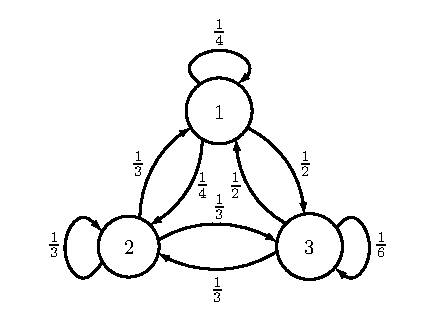
\includegraphics[width=\textwidth]{markov2}
\caption{Transition diagram}
\label{fig:markov2}
\end{figure}

\begin{enumerate}
\item Find the transition matrix.
\item If the Markov process is in state 1 initially, find the probability that it is in state 2 after 2 transitions.
\item Find the stable fixed point if it exists.
\end{enumerate}
\end{problem}